
\chapter{Documenting an API}

``\textbf{API}" -- which historically stands for ``Application Programming
Interface" -- is one of the dumber acronyms you'll encounter. And worse, it's
commonly used to mean two different things: (1) a set of classes (and their
methods) which a programmer could make use of in their own code, and (2) the
documentation describing those classes/methods.\footnote{By the way, the term
``API" isn't used only for object-oriented software. One could write some
old-school procedural code (with functions and data structures, rather than
encapsulated classes and methods), describe it, and call that an API as well.}

In common lingo, people speak of ``programming to an API," which means
``writing some code which conforms to those documented classes/methods." Every
time you've used an \texttt{ArrayList} or a \texttt{Scanner}, in fact, you
have been doing this. Instantiating such objects, calling methods on them, and
(importantly) reading the documentation at
\url{https://docs.oracle.com/javase/8/docs/api/} to find out how they
operate is all part of leveraging the built-in Java API for your own purposes.

These days, when people talk about using an API, they often mean writing code
that connects over the Internet to some publicly-available service or database
of information. Nearly every major Internet player these days -- Google,
Youtube, Instagram, Flickr, eBay, Twitter, Dropbox, Spotify, Amazon,
\texttt{data.gov}, GeoDB cities, \textit{etc.} -- has a publicly-accessible
API. This allows you to write code (in any language) to connect to it and
query it for information, perform commands, make purchases, and so forth.
Browse \url{dev.twitter.com} to get an idea of the rich functionality
available to anyone with the technical savvy to understand and exploit an API.

It's an interconnected, collaborative world. Developers rarely write all the
code themselves anymore, all on an isolated island. Instead, they share code
and for others to use, and take advantage of what's been shared with them. If
you can figure out how to effectively do that, you've increased your
programming potential a hundredfold.

\section{The importance of good documentation}

Now in order to make it possible for other developers to use the code you so
painstakingly wrote, it must be \textbf{documented} in a way that is clear,
complete, and unambiguous. To appreciate the importance of this, I want to
lead you in a thought experiment.

First, pretend you're back in the 1990's, a glorious time to be young and
alive. In particular, pretend that \textit{GPS and cell phones are not yet
commonly available.} (Believe it or not, this was true in the recent past.)

Let's suppose it's Friday night, and you're going to a party at the apartment
of your acquaintance Biff. Biff lives up in North Stafford, and you've never
been to his place before. Luckily, your close friend Filbert is also going to
the party, and he's been to Biff's on many occasions. You're picking him up at
8pm.

Consider the following two scenarios.

\begin{description}

\item[Scenario A:] You'll pick up Filbert (and possibly one or two others), and
drive together to Biff's apartment.

\item[Scenario B:] Filbert calls you at the last minute and says that he's
getting a ride with somebody else. He gives you \textit{written directions} to
Biff's, however, so that you can get to the party on your own.

\end{description}

My question: in which of the above two scenarios are you \textit{more} likely
to successfully arrive at the party without getting lost? Or are both cases
equally likely?

The careless thinker might at first conclude that the two cases are equally
likely. After all, they both depend on Filbert's knowledge of how to get to
Biff's. In one case, Filbert's verbalizing the directions as you drive, and in
the other case, he's laying them all out for you in advance. But
theoretically, as long as Filbert knows how to get there, you'll be successful
in both scenarios.

Theoretically. But in the real world, as everyone knows, it usually doesn't
work like that. In scenario A, and Filbert in the passenger seat, you have the
chance to interactively ask about every intersection and every turn. In
scenario B, \textit{Filbert had to specify everything perfectly in advance.}
He had to describe the route with no errors, since there would be no chance to
make corrections en route. He had to anticipate every question you might have,
since he wouldn't be there to answer them. That's a lot of pressure on Filbert
to give good directions.

Consider the following very realistic possibilities:

\begin{itemize}
\itemsep.1em

\item Filbert wrote ``left" when he meant ``right" in step 3 of the directions
because he's human.

\item Filbert just plain forgot step 5 of the directions because he's human.

\item When he wrote, ``turn left at the next opportunity," he meant ``at the
next intersection," and assumed that would be obvious to you. However, you
quite naturally thought he meant ``the very next possible left," which was
down a side road.

\item A road is closed, or there's a traffic jam, and you need to go around it
in order to make it to the party on time.

\item \textit{Etc.}

\end{itemize}

You can think of a dozen more. In all these cases, having Filbert with you in
the car allows you to clarify ambiguities, fill in omissions, ask questions as
they arise, and change course in response to unexpected circumstances. With
the written directions, you have none of those options. Put another way,
Filbert isn't even at your disposal in Scenario B: your only asset is
Filbert's brain dump, as he was conceiving it at 6:13pm.

And by the way: most people are pretty bad at giving directions.

\subsection{Collaborating with someone you'll never meet}

In case the above analogy isn't plain, Scenario A corresponds to a software
development team where your teammates are just down the hall. They're just an
email or a Slack away. You can ask questions, report bugs, or even request
alterations as the need arises. The pressure is off, as far as documentation
is concerned. In fact, why even bother trying to document everything
exhaustively in advance, if your teammates can ask focused questions in real
time?

Scenario B corresponds to you using a public API. The instructions written by
a developer you will never meet are \textit{your one and only chance} to
comprehend how to use the thing. Those instructions had better be darned good,
because there is no chance to ask questions on the road. They'd better clearly
and exhaustively contain \textit{everything} you're likely to want to know.

By the way: most people are pretty bad at writing clear and complete
documentation. The good news is that it's possible to improve this through
discipline, practice, and painstaking effort.

\section{JavaDoc: mechanics}

One of Java's supplementary (but in retrospect, killer) features was the
\texttt{javadoc} utility shipped with the JDK. 

The idea behind JavaDoc is to combine two previously incompatible aspects of
code documentation. On the one hand, one could argue that the English text
describing how to use a software component (like a class, method, or package)
ought to be maintained right alongside the code itself. This promotes keeping
the two in sync.

On the other hand, there are clearly many advantages to presenting the
documentation in a rich, interactive, point-and-click hypertext format rather
than embedded into plain-text. So we seem to have two conflicting desires: to
keep the documentation close to (and embedded in) the code, and to author it
in a more flexible (and ideally, web-browser-accessible) way outside the code.

JavaDoc's innovation was to say: ``go ahead and store the documentation in the
\texttt{.java} files themselves, to promote consistency. But we'll create a
separate tool that can examine the \texttt{.java} files and extract the
documentation portions. The tool will then assemble those into a mini-website
that other programmers can conveniently browse."

To accomplish this, we use a special syntax to denote ``JavaDoc comments."
Recall that one style of comment in Java is the multi-liner:

\vspace{-.2in}
\begin{Verbatim}[fontsize=\footnotesize,samepage=true,frame=none]
    /*
     * This is a regular Java comment, and will be ignored by javac.
     */
\end{Verbatim}

JavaDoc comments are the same, except that they have a \textit{double}
asterisk at the beginning:

\begin{Verbatim}[fontsize=\footnotesize,samepage=true,frame=none]
    /**
     * This is a special JavaDoc comment, which will be ignored by javac,
     * but will be extracted by javadoc.
     */
\end{Verbatim}

You can place JavaDoc comments in three places:

\begin{itemize}
\itemsep.1em

\item Immediately before a class definition, to provide a description of that
class, and hints as to its usage.

\item Immediately before a method definition, to describe what the method
does, how to call it, and what will happen in exceptional conditions.

\item In a special file called ``\texttt{package.html}", which will be placed
in the source directory for a package, if you're using Java packages.

\end{itemize}

The \texttt{javadoc} utility will automatically identify and extract the
English text stored in JavaDoc comments in any of these three places, and
assemble them into HTML files in the appropriate way.

\subsection{Markup and tags}

There are also a couple of cosmetic options you can take advantage of in
JavaDoc comments. First of all, any valid HTML tag can be used directly in the
comment, and will be formatted appropriately in the final mini-website. If
you're familiar with HTML tags like ``\texttt{$<$b$>$}" (for boldface),
``\texttt{$<$tt$>$}" (for a monospace, typewriter font) or
``\texttt{$<$ul$>$}" and ``\texttt{$<$li$>$}" (for bulleted lists), you can
use them to style your text.

Second, there are special tags called ``JavaDoc tags" that can be used to set
apart certain meta-information and put them in a special place in the final
HTML product. The most important ones are shown in Figure~\ref{fig:taglist},
though there are others. Each development team acquires their own culture,
policies, and procedures that call for different pieces of information to be
highlighted.

\begin{figure}[ht]
\centering
\small
\begin{tabular}{|c|c|l|}
\hline
Tag/syntax & Location & Purpose\\

\hline
\hline

\texttt{@author} \ Jezebel & class & 
\makecell[l]{
The primary or original author of the class.\\
Using the first name, username, or initials of the\\
author are common choices.}\\

\hline

\texttt{@param} \ \texttt{name} \ description & method & 
\makecell[l]{
What one of the arguments to the method means.\\
``\texttt{name}" is either the name or the type of argument.\\
``description" should begin with a lower-case letter\\
and end with a period.}\\

\hline

\texttt{@return} \ description & method & 
\makecell[l]{
How the return value of the method should be\\
interpreted. ``description" should begin with a\\
lower-case letter and end with a period.}\\

\hline

\texttt{@throws} \ type \ description & method & 
\makecell[l]{
What type of exception might be thrown from the\\
method and how it should be interpreted.\\
``description" should begin with the word ``if" and\\
end with a period.}\\

\hline
\texttt{\{@link className\}} & anywhere &
\makecell[l]{
Create a clickable hyperlink to the class named.}\\

\hline

\texttt{\{@link className\#method\}} & anywhere &
\makecell[l]{
Create a clickable hyperlink to the method named.}\\

\hline

\texttt{@deprecated} \ explanation & class/method & 
\makecell[l]{
Mark this class or method as old and not to be used\\
by new code. (Still supported temporarily for older\\
code, but intended to be phased out.)}\\

\hline

\end{tabular}
\vspace{.1in}
\caption{Some commonly-used JavaDoc tags, and their meanings.}
\label{fig:taglist}
\end{figure}
\normalsize

A representative example showing many of these tags is in
Figure~\ref{fig:javadocTags}, the HTML for which appears in
Figure~\ref{fig:javadocApi}.

\begin{figure}
\begin{Verbatim}[fontsize=\footnotesize,samepage=true,frame=single]
/**
 * A <tt>Ballplayer</tt> represents a historical baseball player and the
 * composite statistics over his career. Each <tt>Ballplayer</tt> object
 * is associated with one {@link Team} even if he played for multiple
 * teams in his actual career.
 * @author SD
 */
public class Ballplayer {
    ...
    /**
     * Constructs a new <tt>Ballplayer</tt> object with "empty" stats
     *   (<i>i.e.</i>, all set to their initial, default values.)
     * @param name the real (no nicknames) first and last name of the player.
     * @param uni the most well-known uniform number he played under.
     * @param team the mascot name (not city) of the {@link Team} he is most
     *   commonly associated with.
     * @throws NoTeamException if the <tt>team</tt> parameter does not
     *   correspond to the mascot name of any known {@link Team}.
     */
    public Ballplayer(String name, int uni, String team) throws NoTeamException {
        ...
    }
    
    /**
     * Returns the player's career batting average, measured as total hits
     *   divided by total "at bats." If the number of "at bats" is zero,
     *   returns 0.0 rather than give a divide-by-zero error.
     * @deprecated This method should be eschewed in favor of more recently
     *   developed stats such as {@link Ballplayer#getOnBasePercentage} and
     *   {@link Ballplayer#getSluggingPercentage}.
     * @return the batting average on a 0.0-to-1.0 scale.
     */
    public double getBattingAvg() {
        ...
    }
}
\end{Verbatim}

\caption{HTML and JavaDoc tags in action.}
\label{fig:javadocTags}
\end{figure}


\subsection{Generating the mini-website}

To actually generate the HTML in Figure~\ref{fig:javadocApi}, you'll need to
run the \texttt{javadoc} command with some options. Generally, if I'm running
on a Google Cloud instance, this is how I run it:

\begin{Verbatim}[fontsize=\small,samepage=true,frame=none]
$ sudo javadoc -d /var/www/html -author *.java
\end{Verbatim}

The word ``\texttt{sudo}" at the start of this sentence means ``please allow
me to execute the following command as the \textbf{root} user of the system";
\textit{i.e.}, the super user who has all privileges. The reason this is
necessary is that the directory \texttt{/var/www/html}, which this command
says to write content in, is by default not writeable by ordinary mortals. You
have to temporarily become Superman in order to write to it, which will
require typing your password to confirm you're really Clark Kent.

The ``\texttt{-d /var/www/html}" bit is a command option with a parameter. The
\texttt{-d} stands for ``directory" and it says that the HTML that
\texttt{javadoc} generates should be written to this directory. It's a
system-specific thing; on Debian Linux (which I install on Google Cloud) this
is the directory that Apache Web Server will look in to serve up content to
browsers that connect to it. (More on that in a moment.) In other contexts,
like if you have a user directory on a shared machine that you don't have
control over, you can often substitute something like ``\texttt{-d
/home/yourusername/public\_html}" which will write the content to your
account's own directory for hosting HTML content to the world.

The ``\texttt{-author}" part of the command says ``yes, please \textit{do}
extract \texttt{@author} information and include it in the HTML. (The default
is to not do that, which I've never understood.) Semi-related: by default
\texttt{javadoc} only includes the \textbf{public} classes and methods in the
HTML it generates, since JavaDoc is normally used to document public APIs.
Sometimes there are reasons to produce JavaDoc content for \textit{everything}
in the class files -- private, public, or anything else -- and to do this you
merely need to include a ``\texttt{-private}" option here as well.

Finally, the ``\texttt{*.java}" means to generate HTML for all the Java source
files in the current directory. If you're using packages, you can instead
replace ``\texttt{*.java}" with a sequence of fully-specified package names
that can be located via the \texttt{CLASSPATH} variable. Note that you
do have to tell \texttt{javadoc} to generate the \textit{entire} mini-website
at once; if you make just a change or two to one \texttt{.java} file, you
can't just regenerate the HTML for that one because then the entire
mini-website will consist of nothing \textit{but} that one class.

\subsubsection{Starting the Web server and connecting}

After all the JavaDoc's mini-website content has been generated, you can
access it via your browser. You can find out whether Apache Web Server is
running by typing:

\begin{Verbatim}[fontsize=\small,samepage=true,frame=none]
$ sudo systemctl status apache2
\end{Verbatim}

at the command line. If it gives a message like ``whoa, apache2 not
installed," then you'll need to install it via:

\begin{Verbatim}[fontsize=\small,samepage=true,frame=none]
$ sudo apt install apache2
\end{Verbatim}

If it says it's not currently running, then you'll need to start it via:

\begin{Verbatim}[fontsize=\small,samepage=true,frame=none]
$ sudo systemctl start apache2
\end{Verbatim}

Lastly, when this seems to be working, figure out what the external IP address
is of your machine (it'll be four numbers, each in the range 0-255, set apart
by periods; for example, 35.237.255.14). Then, you can point your browser to
\url{http://thatIPAddress} and you should be able to see your
prettily-formatted HTML website like in Figure~\ref{fig:javadocApi}.




\begin{figure}
\centering
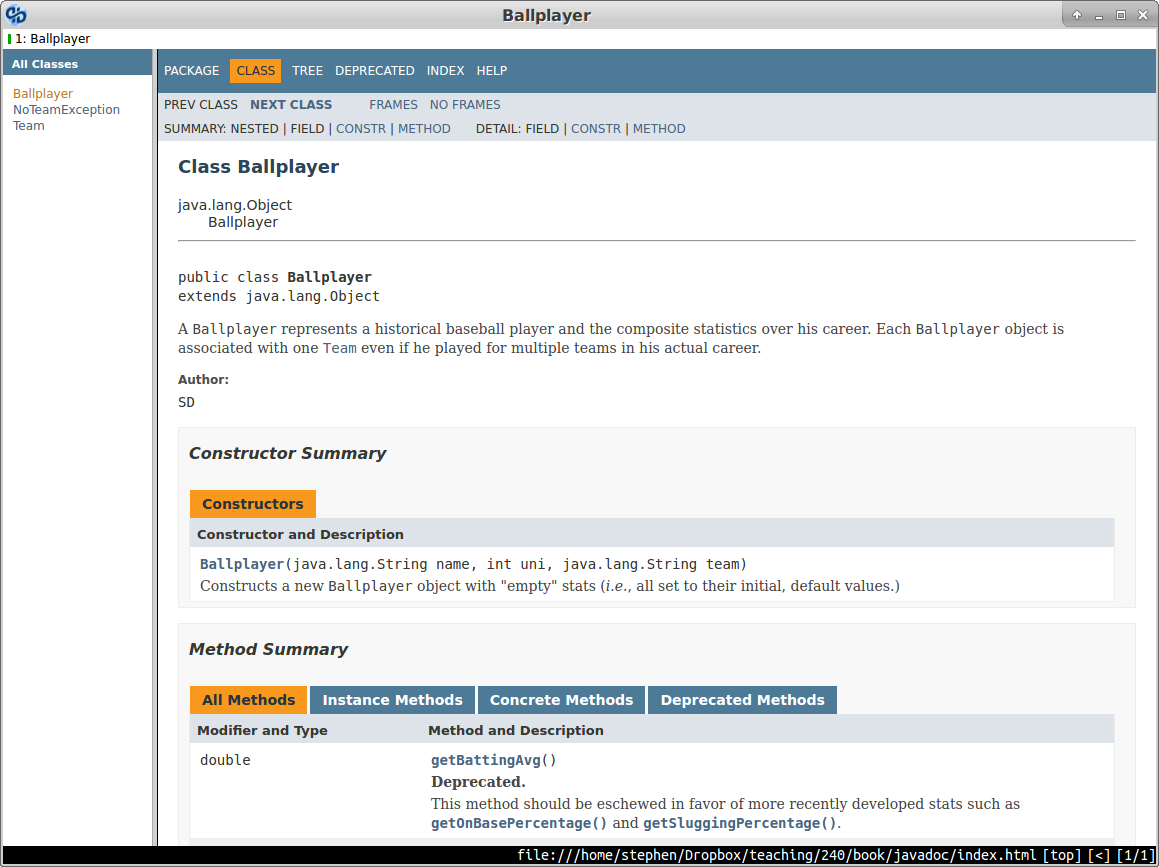
\includegraphics[width=0.9\textwidth]{javadoc1.png}

\vspace{.1in}

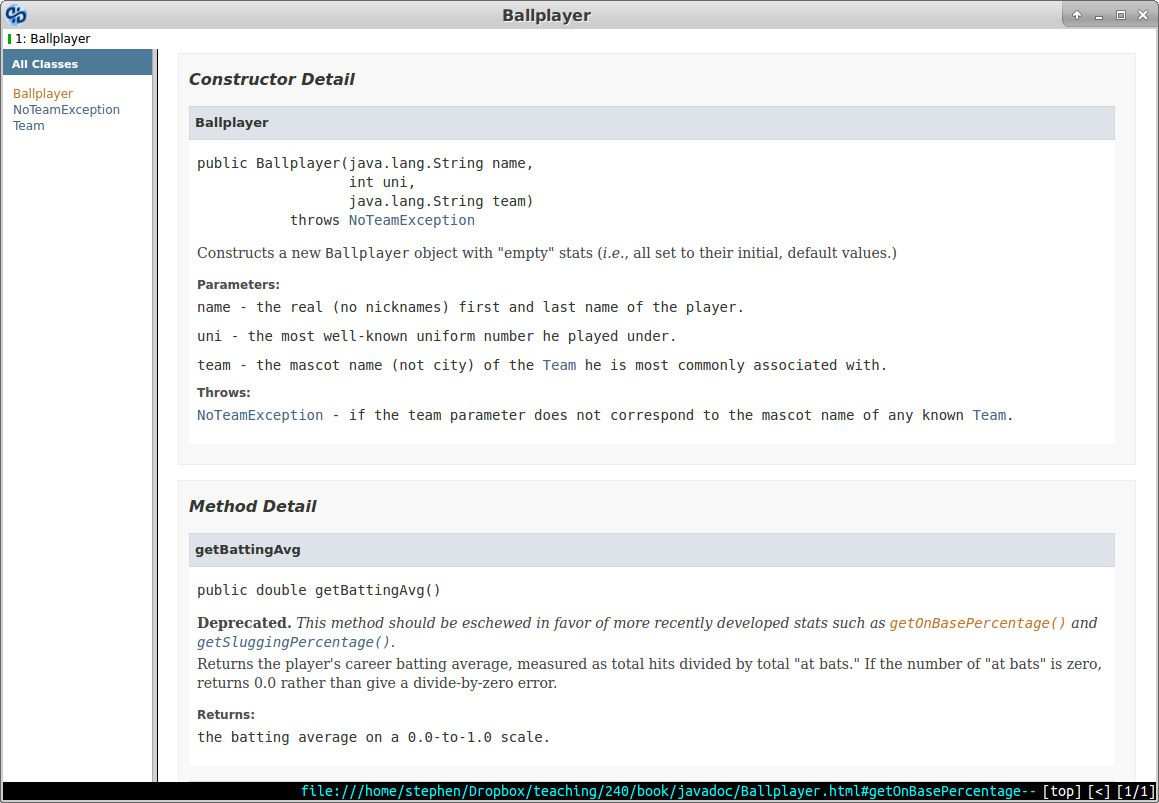
\includegraphics[width=0.9\textwidth]{javadoc2.png}

\vspace{.1in}

\caption{The generated HTML for the code in Figure~\ref{fig:javadocTags}.}
\label{fig:javadocApi}
\end{figure}


\section{JavaDoc: content}

Okay, so that's all the minutiae of how to get the JavaDoc syntax right and
generate the website. You have to know it, but it's not the important part.
The truly important question in all this is less-easily defined: how to
actually write quality documentation that will communicate effectively to
programmers I may never meet?

